\documentclass{article}
\usepackage{amsmath, sfmath, multicol, tkz-euclide, array, enumerate, tcolorbox, tabularray}
\renewcommand{\familydefault}{\sfdefault}
\setlength{\parindent}{0cm}
\pagestyle{empty}
\usepackage[left=1in, top=0.5in, right=1in, bottom=0.5in]{geometry}
\tikzset{>=stealth}
\tcbset{colback=white}

\newcounter{example}[section]
\newenvironment{example}[1][]{\refstepcounter{example}\par\medskip
   {\color{red}\textbf{Example~\theexample. #1}}}{\medskip}

\begin{document}

\section*{Perimeter and Area of Similar Figures}

\begin{tcolorbox}[colframe=orange!70!white, coltitle=black, title=\textbf{Today I Can}]
\begin{enumerate}
    \item Find perimeters and areas of similar polygons.
\end{enumerate}
\end{tcolorbox}
\smallskip

\begin{example}
Answer the following given the diagram. \newline 

\begin{minipage}{0.4\textwidth}
\begin{tikzpicture}[scale=0.7]
\draw (0,0) rectangle (2,1);
\node at (1,0) [anchor = north] {5};
\node at (0,0.5) [anchor = east] {2};
\node at (2,0.5) [anchor = west] {2};
\node at (1,1) [anchor = south] {5};
\end{tikzpicture}
\hspace{0.25in}
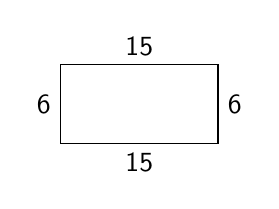
\begin{tikzpicture}
\draw (0,0) rectangle (2,1);
\node at (1,0) [anchor = north] {15};
\node at (0,0.5) [anchor = east] {6};
\node at (2,0.5) [anchor = west] {6};
\node at (1,1) [anchor = south] {15};
\end{tikzpicture}
\end{minipage}
\begin{minipage}{0.5\textwidth}
\begin{enumerate}[(a)]  \setlength{\itemsep}{20pt}
    \item What is the ratio of corresponding sides?
    \item What is the perimeter of each rectangle?
    \item What is the ratio of perimeters (smaller to larger)?
    \item What is the area of each rectangle?
    \item What is the ratio of areas (smaller to larger)?
\end{enumerate}
\end{minipage}
\end{example}
\vspace{1.5cm}

\begin{tikzpicture}
\draw (0,0) rectangle (14, 2);
\node [left] at (0,1) {\textbf{Main Ideas:}};
\end{tikzpicture}

\vspace{0.5in}

\begin{example}
The area of the smaller regular pentagon is about 27.5 cm$^2$. What is the best approximation for the area of the larger regular pentagon?
\newline\\

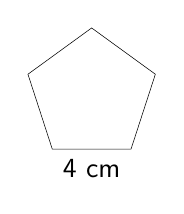
\begin{tikzpicture}
\tkzDefPoints{0/0/A, 1/0/B}
\tkzDefShiftPoint[A](108:1){E}
\tkzDefShiftPoint[B](72:1){C}
\tkzDefShiftPoint[E](36:1){D}
\tkzDrawPolygon(A,B,C,D,E)
\tkzLabelSegment[below](A,B){4 cm}
\end{tikzpicture}
\hspace{0.25in}
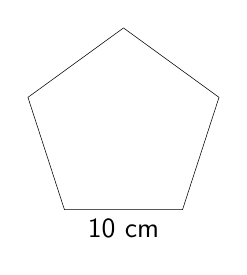
\begin{tikzpicture}[scale=1.5]
\tkzDefPoints{0/0/A, 1/0/B}
\tkzDefShiftPoint[A](108:1){E}
\tkzDefShiftPoint[B](72:1){C}
\tkzDefShiftPoint[E](36:1){D}
\tkzDrawPolygon(A,B,C,D,E)
\tkzLabelSegment[below](A,B){10 cm}
\end{tikzpicture}
\end{example}

\newpage 

\begin{example}
The scale factor of the dimensions of 2 similar pieces of window glas is 3 : 5.    \newline

What is the cost of the larger piece?   \newline

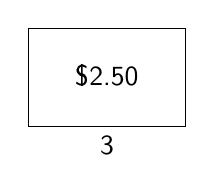
\begin{tikzpicture}
\draw (0,0) rectangle (2,1.25);
\node at (1,0) [anchor = north] {3};
\node at (1,0.65) {\$2.50};
\end{tikzpicture}
\hspace{0.25in}
\begin{tikzpicture}
\draw (0,0) rectangle (3, 1.75);
\node at (1.5,0) [anchor = north] {5};
\end{tikzpicture}
\end{example}

\vspace{2in}

\begin{example}
The triangles shown are similar.    \newline

\begin{minipage}{0.5\textwidth}
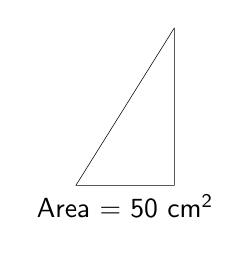
\begin{tikzpicture}
\tkzDefPoints{0/0/A, 1.25/0/B, 1.25/2/C}
\tkzDrawPolygon(A,B,C)
\tkzLabelSegment[below](A,B){Area = 50 cm$^2$}
\end{tikzpicture}
\hspace{0.25in}
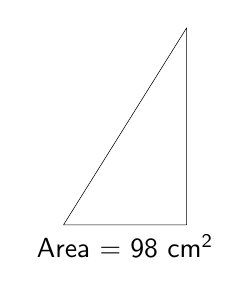
\begin{tikzpicture}[scale=1.25]
\tkzDefPoints{0/0/A, 1.25/0/B, 1.25/2/C}
\tkzDrawPolygon(A,B,C)
\tkzLabelSegment[below](A,B){Area = 98 cm$^2$}
\end{tikzpicture}
\end{minipage}
\begin{minipage}{0.4\textwidth}
\begin{enumerate}[(a)]
    \item What is the scale factor (smaller to larger)? \\[0.75in]
    \item What is the ratio of their perimeters?
\end{enumerate}
\end{minipage}
\end{example}


\end{document}
